\section{First Problem}

\subsection{Problem Statement}

Suppose we have a functional:
\begin{equation}
    J[u(x,y)]=
    \iint_B
    \left[
        \left(
            \frac{\partial u}{\partial x}
        \right)^2+
        \left(
            \frac{\partial u}{\partial y}
        \right)^2 - 2u
    \right]dxdy
\end{equation}

And boundary condition:
\begin{equation}
    u|_{\partial B} = 0
\end{equation}

where $B$ is a domain in $x-y$ plane enclosed by:
\begin{equation}
    y=\pm \frac{\sqrt{3}}{3}x\quad\text{and}
    \quad x=b
\end{equation}

Let the functional achieve the minimum value.

\begin{enumerate}[(1)]
    \item Write the equivalent governing equation in the domain.
    \item Programming: use finite element method to solve the field $u$ within the domain 
    numerically. In the report, please make a brief description of your code, and illustrate 
    the validity of your results. (Please attach the code in another file.)
\end{enumerate}

\subsection{Governing Equation}

In $J[u(x,y)]$, the part
$$
    \left(
            \frac{\partial u}{\partial x}
        \right)^2+
        \left(
            \frac{\partial u}{\partial y}
        \right)^2
$$
can be written as:
\begin{equation}
    \left(
            \frac{\partial u}{\partial x}
        \right)^2+
        \left(
            \frac{\partial u}{\partial y}
        \right)^2
        =\nabla u\cdot \nabla u
\end{equation}

thus $J[u(x,y)]$ can be written as:
\begin{equation}
    J[u(x,y)]=
    \int_B (\nabla u\cdot \nabla u - 2u)d\Omega
\end{equation}

considering the expression below:
$$
\int_B u\nabla^2u d\Omega
$$

use integrate by part and divergence theory we will have:
\begin{equation}
    \begin{aligned}
        \int_B u\nabla^2u d\Omega
        &=\int_B u(\nabla\cdot \nabla u)d\Omega\\
        &=\int_{\partial B} u\nabla u \cdot \vec{n} ds
        -
        \int_B \nabla u\cdot \nabla u d\Omega
    \end{aligned}
\end{equation}

at the boundary we have $u|_{\partial B} = 0$, thus we have:
\begin{equation}
    \int_B \nabla u\cdot \nabla u d\Omega
    =-
    \int_B u\nabla^2u d\Omega
\end{equation} 


denote the operator as below:
\begin{equation}
    (u,v) = \iint_B uv dxdy = \int_B uv d\Omega
\end{equation}

thus $J[u(x,y)]$ can be written as:
\begin{equation}
    \label{Ju1}
    \begin{aligned}
        J[u(x,y)]&=
    - \int_B u(\nabla^2 u + 2) d\Omega
    \\
    &=-(\nabla^2 u+2,u)\\
    &=(-\nabla^2 u -2, u)
    \end{aligned}
\end{equation}

for the governing equation $Au=f$ the $J[u]$ is as below:
\begin{equation}
    \label{Ju2}
    Ju = (Au-2f,u)
\end{equation}

compare eq.\ref{Ju1} with eq.\ref{Ju2} we get the governing equation ($A=-\nabla^2 , f=1$):
\begin{equation}
    -\nabla^2 u=1
\end{equation}

\subsection{FEM Method in Triangle Mesh}

Devide the domain $B$ into a large number of triangle mesh cells, 
and use interpolation to get the value of $u$ inside cells through the 
node value of each triangle cell. 
Now suppose we have a triangle cell called $\Omega$, which possesses $3$ nodes called 
$1,2,3$. 
The value of $u$ on these nodes are called $u_j(j=1,2,3)$.
Thus the approximate value of $u$ inside the cell called $\tilde{u}$ can be written as:
\begin{equation}
    \tilde{u}=\sum_{j=1}^3 \phi_j u_j
\end{equation}

use galerkin method we have in the cell $\Omega$ we have:
\begin{equation}
    \int_\Omega (A\tilde{u}-f) \phi_i d\Omega  = 0\quad i=1,2,3
\end{equation}

in this case let $A=-\nabla^2,f=a=1$, we have:
\begin{equation}
    \int_\Omega (\nabla^2\tilde{u} + a)\phi_i d\Omega=0 \quad i=1,2,3
\end{equation}

which is exactly:
\begin{equation}
    \sum_{j=1}^3 u_j\int_\Omega \phi_i\nabla^2\phi_j d\Omega
    +
    a\int_\Omega \phi_i d\Omega = 0
\end{equation}

the part $\int_\Omega \phi_i\nabla^2\phi_jd\Omega$ can be written as:
\begin{equation}
    \label{galerkin}
    \int_\Omega \phi_i\nabla^2\phi_jd\Omega
    =
    \int_{\partial \Omega}\phi_i\nabla \phi_j\cdot \vec{n}ds-
    \int_\Omega \nabla\phi_i\cdot\nabla\phi_j d\Omega
\end{equation}

for the value $\phi_i\nabla\phi_j\cdot\vec{n}$ will be compensated by the cell 
opposite this edge, we can negelect this part, thus eq.\ref{galerkin} turn to be:
\begin{equation}
    \sum_{j=1}^3
    u_j
    \int_{\Omega}\nabla\phi_j\cdot\nabla\phi_i d\Omega
    =
    a\int_\Omega \phi_i d\Omega
\end{equation}

in vector form that is:
\begin{equation}
    \begin{bmatrix}
        \int_\Omega\nabla\phi_i\cdot\nabla \phi_1d\Omega
        &
        \int_\Omega\nabla\phi_i\cdot\nabla \phi_2d\Omega
        &
        \int_\Omega\nabla\phi_i\cdot\nabla \phi_3d\Omega
    \end{bmatrix}
    \begin{bmatrix}
        u_1\\u_2\\u_3
    \end{bmatrix}=
    a\int_\Omega \phi_i d\Omega
\end{equation}

in triangle mesh the function $\phi_k$ is known, denote $2A$ as:
\begin{equation}
    2A=
    \begin{vmatrix}
        1 & x_1 & y_1\\
        1 & x_2 & y_2\\
        1 & x_3 & y_3
    \end{vmatrix}
\end{equation}

thus $\phi_1\sim \phi_3$ is:
\begin{equation}
    \phi_1=
    \frac{
        \begin{vmatrix}
            1 & x & y\\
            1 & x_2 & y_2\\
            1 & x_3 & y_3
        \end{vmatrix}
    }{2A}
    \quad
    \phi_2=
    \frac{
        \begin{vmatrix}
            1 & x_1 & y_1\\
            1 & x & y\\
            1 & x_3 & y_3
        \end{vmatrix}
    }{2A}\quad
    \phi_3=
    \frac{
        \begin{vmatrix}
            1 & x_1 & y_1\\
            1 & x_2 & y_2\\
            1 & x & y
        \end{vmatrix}
    }{2A}
\end{equation}

here the order of node $1,2,3$ should be anti-clockwise.
Finally we just need to add the part matrix into the general matrix to attain:
\begin{equation}
    [K]u=b
\end{equation}

the $u$ at the boundary is known as zero, thus we need to cut the matrix $[K]$ into a 
smaller one. The value of $u$ at nodes inside the domain can be calculated by the 
inversion of the modified $[K]$ and modified $b$. Denote the modified $[K]$ after removing
 the boundary elements as $[K]_m$ and modified $b$ as $b_m$, the $u_m$ is exactly:
\begin{equation}
    u_m = [K]_m^{-1}b_m
\end{equation}

Thus through interpolation we get the distribution of $u$ over the domain $B$.


\subsection{Programming: Julia Code}

For this work, I choose to use Julia language to finish the task. 
I will explain the procedure of my codes as below.

\subsubsection{Mesh Part}

The FEM method depends on the triangle mesh. 
I choose to use Mathematica software to generate of mesh.
When $b=1$, the geometry of the domain and the triangle mesh figure is shown 
as below in \ref{Triangle mesh generated by Mathematica}. 
This mesh contains $22689$ nodes and $44895$ cells.

\begin{figure}[H]
    \centering
    \subfloat[Matplotlib Plot]{
        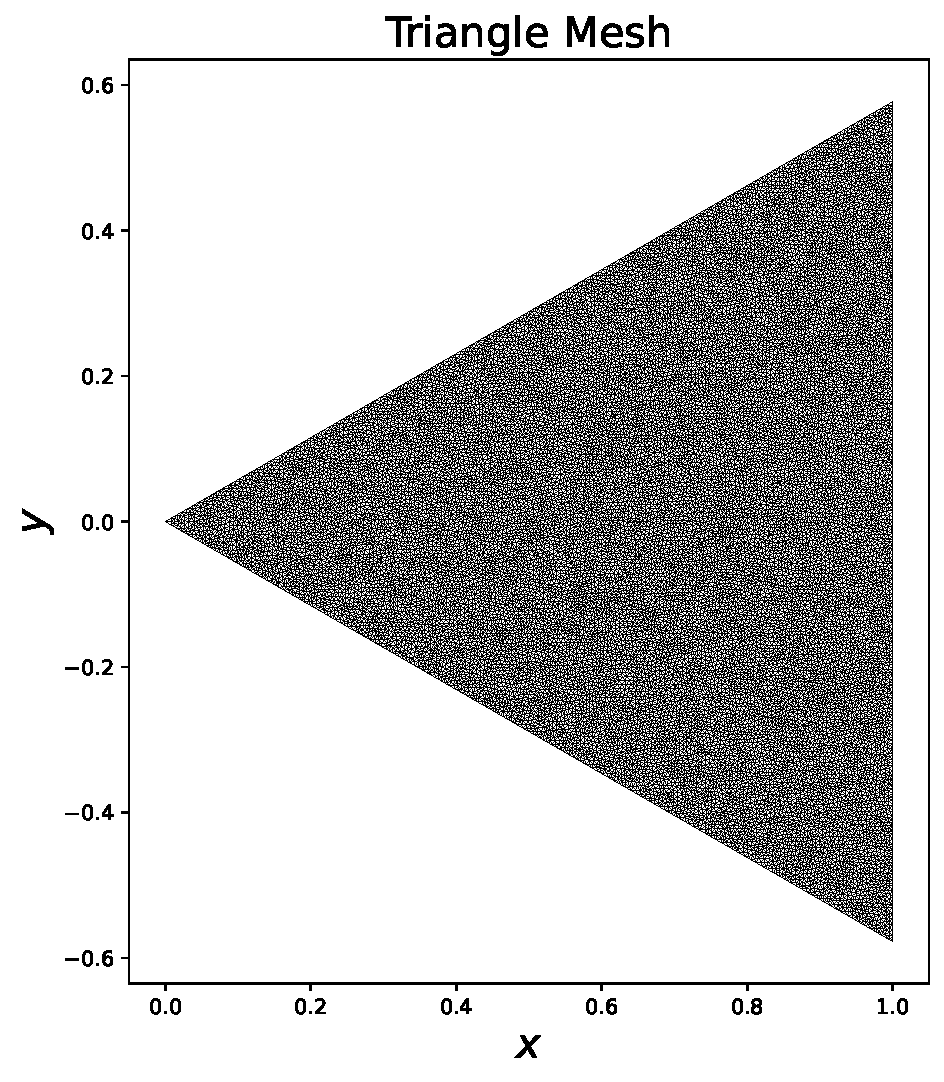
\includegraphics[width=0.45\textwidth]{..//problem1/image/mesh_figure.pdf}
    }\quad
    \subfloat[Mathematica Plot]{
        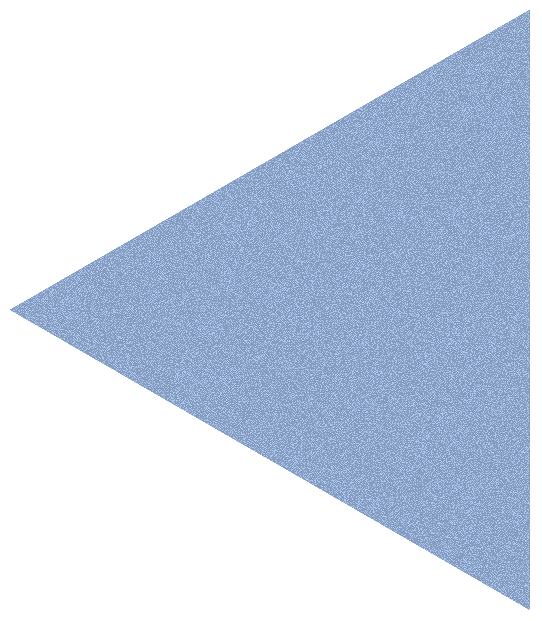
\includegraphics[width=0.45\textwidth]{..//problem1/image/mesh_mma.pdf}
    }
    \caption{Triangle mesh generated by Mathematica}
    \label{Triangle mesh generated by Mathematica}
\end{figure}

In the path 'src', a julia file 'Mesh.jl' is used to read and store the mesh information. 
Here is the component of code in this file.
\begin{enumerate}
    \item readfile\_Vector\_String: function, used to read a file as string vector;
    \item readMatrix: function, used to read data from file as a matrix;
    \item read\_mesh\_ply: function, used to read the mesh information; In addition, the mesh format should be 'ply' which generated from mma;
    \item Mesh: struct, which contains:
    \begin{itemize}
        \item nnodes: number of nodes;
        \item ncells: number of triangle cells;
        \item xy: the $(x,y)$ of nodes;
        \item icell: the connection information of each triangle's nodes;
    \end{itemize}
    \item Mesh: function, used to generate a Mesh struct from mesh file.
\end{enumerate}

\subsubsection{Case Part}

This part is contained in file 'src//Case.jl' including:
\begin{enumerate}
    \item Case: struct, used to set the calculation case including:
    \begin{itemize}
        \item alpha: the angle $\alpha$ which is default as $30^\circ$;
        \item b: the domain decided by $x=b$ which is default as $1$;
        \item a: the governing equation as $-\nabla^2 u = a$ which is default as $1$;
        \item boundary\_value: the value of $u$ on boundary which is default as zero.
    \end{itemize}
    \item Case: function, generate a default calculation case;
    \item whether\_on\_boundary: function, to judge whether $(x,y)$ is on the boundary of the calculation case.
\end{enumerate}

\subsubsection{Solver Part}

This part is contained in file 'src//Solver.jl' used to solve the problem including:
\begin{enumerate}
    \item generate\_K\_b: function, to generate $[K]$ and $b$ from case and mesh;
    \item boundary\_node\_ID: function, to mark the node at the boundary and store their IDs;
    \item solve: solve the value $u$ at each node.
\end{enumerate}

It's noteworthy that julia has amazing speed in loop and matrix inversion. 
Here for the matrix $[K]$ is a sparse large scale matrix, 
I use a package 'SparseArrays' to store $[K]$. 
This saves much memory and the inversion progress is done by 'MKL', 
the total solution only costs about $20$ seconds.

\subsubsection{Main Part}

This part is contained in file 'src//Main.jl' used to set the case, read the mesh, 
solve the problem and draw the contour of result. 
Here I use 'PyPlot' package to call matplotlib to draw the contour of distribution of $u$. 
For I write detailed code annotation in this file, I'm not going to expalin it here in the report.

\subsubsection{The Explaination of Working Directory}

The 'problem1' directory contains four sub-directories:
\begin{enumerate}
    \item data: contains mesh file 'mesh.ply' and Mathematica notebook file 'task1.nb' which include the validation of problem 1, generation of mesh and Formula derivation. Moreover, to avoid Mathematica not available on your computer, I print the MMA notebook as a pdf;
    \item image: contains the figures plot by my julia code and Mathematica code;
    \item src: contains my julia FEM code;
    \item draft: some test jupyter notebook files.
\end{enumerate}

\subsection{Result: Contour of the Julia Code Solution}

With help of the api function 'tricontourf' in matplotlib, 
I draw the contour of $u$ by julia code in fig.\ref{julia code solution}.

\begin{figure}[H]
    \centering
    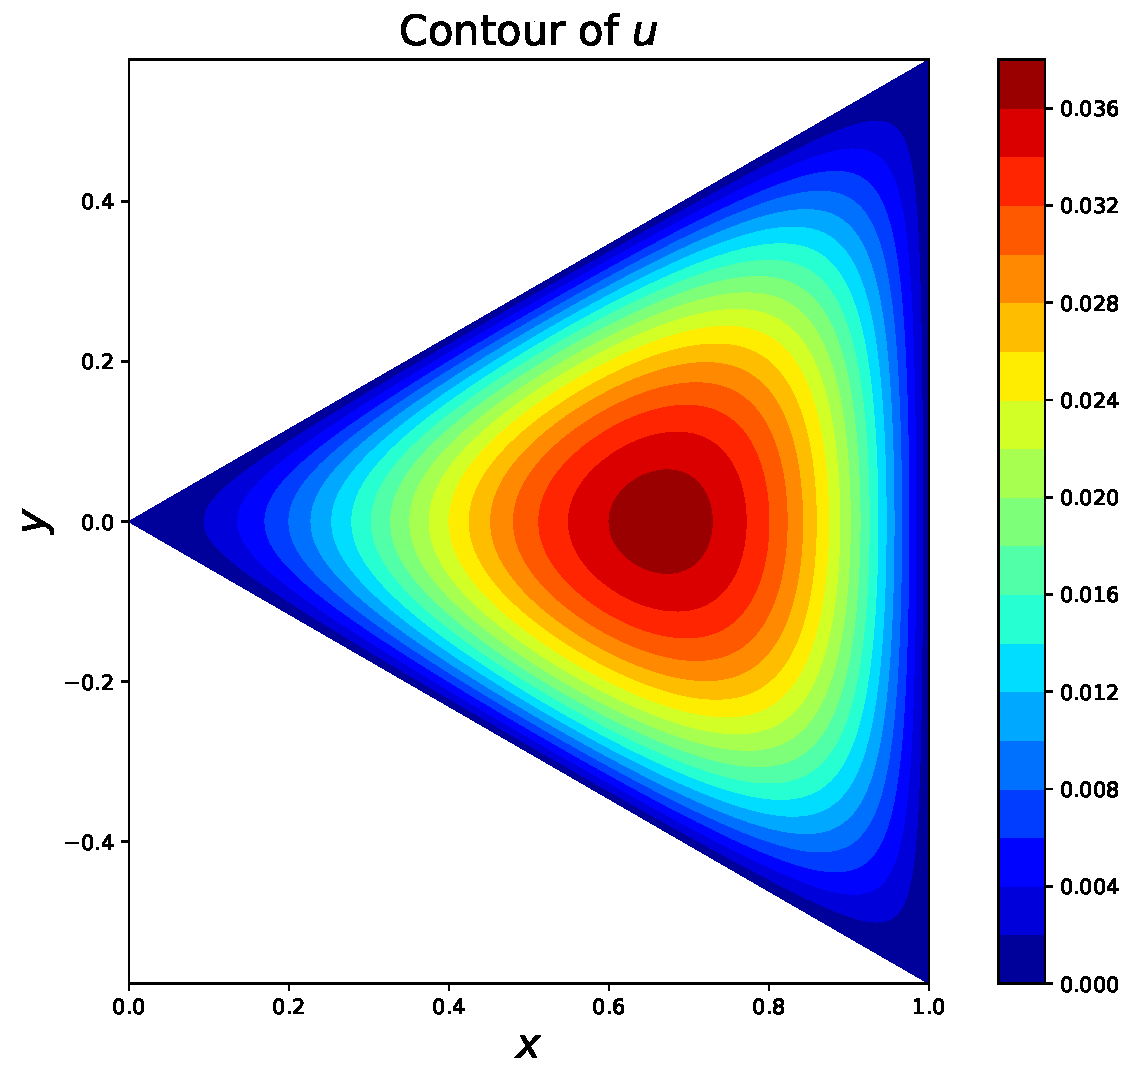
\includegraphics[width=0.55\textwidth]{..//problem1/image/solution_julia.pdf}
    \caption{Contour of $u$ of julia code solution}
    \label{julia code solution}
\end{figure}

\subsection{Validation: Comparison with Mathematica Solution}

\begin{figure}[H]
    \centering
    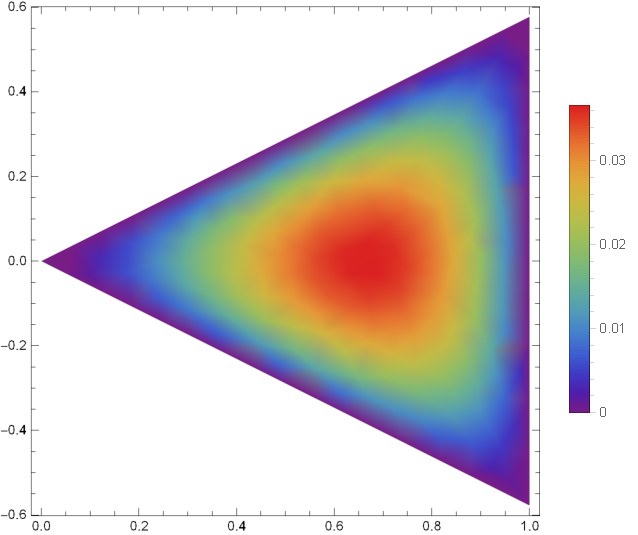
\includegraphics[width=0.55\textwidth]{..//problem1/image/solution_mma.pdf}
    \caption{Contour of $u$ of Mathematica solution}
    \label{mma solution}
\end{figure}

Mathematica is powerful in solveing PDE, 
such problem can be done within several lines of code. 
With MMA, I define the domain and set the governing equation as well as boundary condition, 
the numerical solution of the problem is shown in fig.\ref{mma solution}.

In fig.\ref{julia code solution} and fig.\ref{mma solution} we can easily find that 
the contour of $u$ is the same. 
The red part is in the domain center where $u$ is around $0.03$, 
and the blue part is near the boundary where $u$ is zero as the boundary value. 

This comparison with Mathematica validate the correction of my julia code. 
All these files can be found in directory 'problem1'.